% ================================================================
%  main.tex  --  Quantum-Compatible Drone-VRP (arXiv v1)
% ================================================================
\documentclass[11pt]{article}      % or IEEEtran, lncs, revtex4, etc.

% ---------- Preamble -------------------------------------------------
\usepackage[margin=1in]{geometry}
\usepackage{amsmath,amsfonts,amssymb}
\usepackage{siunitx}           % \SI units
\usepackage{graphicx}
\usepackage{subcaption}        % for subfigures
\usepackage{booktabs}          % nice tables
\usepackage{algorithm}
\usepackage{algpseudocode}
\usepackage{hyperref}
\usepackage{bbm}
\hypersetup{colorlinks, citecolor=blue, linkcolor=blue}

% ---------- Title & Author ------------------------------------------
\title{A Compressed-Qubit, Risk-Aware Quantum Pipeline\\
       for the Drone Vehicle Routing Problem}
\author{%
  Gordon Ma\quad
  Dimitris G. Angelakis \footnotemark[1]
}
\date{\today}

% ---------- Document -------------------------------------------------
\begin{document}
\maketitle
% \begin{abstract}
%   \input{sections/abstract}
% \end{abstract}

% ---------- Main Sections -------------------------------------------
\section{Introduction}

Same-day delivery has evolved from a niche premium into a widespread expectation.
In urban logistics, providers now face pressures to achieve sub-hour deliveries,
dramatically escalating operational complexity.
This urgency intensifies last-mile logistics—which already constitute more than 50\%
of total fulfillment costs—and clashes with increasing demands for carbon efficiency,
sustainability, and regulatory compliance.\footnote{``Urban Fulfillment Outlook 2025,'' DHL Report, 2024.}
Autonomous drone fleets represent a compelling solution to these challenges,
with pilot programs by UPS Flight Forward, Zipline, and Wing demonstrating their
potential to deliver small parcels rapidly while significantly reducing labor and
carbon emissions \cite{murray_multiple_2020}.
Despite this promise, widespread commercialization remains elusive, largely due to
the complex optimization challenges inherent in scaling from controlled pilots to
real-world deployment.

Practical drone logistics at scale involve combinatorial optimization problems with enormous
search spaces and complex, intertwined constraints such as battery limits, no-fly zones,
wave-based launch schedules, and tight customer time windows.
While exact optimization methods such as Mixed-Integer Linear Programming (MILP) or Branch-and-Price
can theoretically solve these problems, industry experience consistently identifies the dominant bottleneck
as the extensive human effort required to model and refine these optimization scenarios,
rather than solver runtime \cite{hildebrandt_implementation_1981,boschetti_contemporary_2024,kallrath_mixed_2000}.
This modeling overhead—requiring specialized expertise to define, tune, and refine optimization
models—often proves prohibitively expensive in real-world deployments.
Consequently, drone logistics providers frequently resort to heuristic methods,
sacrificing optimality to circumvent this modeling burden.

Quantum computing has simultaneously emerged as a potential remedy,
offering a different paradigmatic approach for addressing large-scale combinatorial optimization problems.
Yet initial quantum implementations of drone-routing and similar Vehicle Routing Problems (VRP)
using standard Quadratic Unconstrained Binary Optimization (QUBO) encodings quickly encounter severe limitations:
a modest four-node scenario already demands hundreds of binary variables after MILP linearization, despite the efforts to reduce variable-count,
exceeding current quantum hardware capabilities \cite{davies_quantum_2024}. 

To address this qubit explosion, a diverse family of \emph{qubit-efficient encoding schemes} has recently emerged.
Minimal encodings introduced by Tan et al.~\cite{tan_qubit-efficient_2021}, 
and subsequently refined by Huber et al. for a domain-specific transaction settlement problem ~\cite{huber_exponential_2024} and Leonidas et al. for vehicle routing problem with time windows for shipping logistics ~\cite{leonidas_qubit_2024}, 
compress resources exponentially by encoding each variable within the Bloch sphere and extracting correlations through register projections.
However, these methods inherently remain a mean-field linear-relaxation heuristic,
which can incur worst-case integrality gaps of at least 2x on canonical combinatorial problems such as Max-Cut~\cite{charikar_integrality_2009}.
Pauli-Correlation Encoding (PCE), proposed by Sciorilli et al.~\cite{sciorilli_towards_2025}, 
captures higher-order Pauli correlations but optimizes a non-convex \(\tanh\) surrogate objective, 
without clear connections to established LP or SDP relaxations.
Meanwhile, the qubit-efficient Quantum Approximate Optimization Algorithm (QAOA) by Sundar and Dupont~\cite{sundar_qubit-efficient_2024} 
maps \(N\) classical bits onto \(q = d + \log_2(N/d)\) qubits, demonstrating parameter clustering on spin-glass instances, 
but remains limited by sampling from depth-\(p\) circuits.
In essence, these advanced encoding methods typically seek single bit-string solutions, 
trading circuit depth and non-convexity challenges for reduced qubit count, yet still fail to fully escape
limitations in practical scaling and constraint management.

An alternative, complementary approach gaining traction is the integration of quantum components as
probabilistic, risk-aware samplers embedded within sophisticated classical preprocessing workflows.
Recent advances frame the quantum device as part of a hybrid quantum-classical optimization loop,
explicitly shifting feasibility management to classical preprocessing while allowing quantum
hardware to specialize purely on combinatorial subset selection \cite{matsuyama_sampling-based_2025}.
Such hybrid pipelines naturally incorporate modern AutoML techniques like Bayesian optimization (Optuna),
which systematically replace manual parameter tuning, 
making them especially appealing for practical industry deployment \cite{akiba_optuna_2019,tibaldi_bayesian_2023,caramanis_optimizing_2023}.

\textbf{Our approach and contributions.} 
In this paper, we introduce a novel hybrid quantum-classical optimization framework specifically tailored for drone logistics,
that leverages advanced classical preprocessing to rigorously manage feasibility constraints,
leaving quantum hardware to specialize purely on subset selection using minimal qubit resources.
Our approach first employs a greedy soft-max heuristic to generate a manageable pool of feasible drone routes,
which are then encoded compactly using just 13 qubits via logarithmic indexing.
By integrating Bayesian hyperparameter optimization (Optuna's Tree-Parzen Estimator) 
with a Conditional-Value-at-Risk (CVaR)-optimized Variational Quantum Eigensolver (VQE),
we demonstrate a robust 6–8\% cost reduction over a Genetic Algorithm baseline—a strong,
reliable solver widely adopted in industry scenarios where custom-crafted optimization
solutions are impractical or prohibitively costly.

The key contributions of this work are as follows:
\begin{enumerate}
\item The first quantum-classical logistics pipeline explicitly designed to minimize both human modeling overhead and qubit count simultaneously.
\item Demonstrated quantum advantage in a real-world-inspired logistics problem, using a CVaR optimization strategy and minimal encoding to achieve superior results over established industry-relevant heuristics.
\item A comprehensive, reproducible open-source toolkit facilitating immediate community adoption and further exploration of hybrid quantum-classical optimization methods in logistics.
\end{enumerate}

The remainder of the paper is structured as follows. 
In Section~\ref{sec:related_work}, we situate our contributions within existing approaches and recent developments in quantum optimization methods.
Section~\ref{sec:problem} rigorously defines the Subset-Route Drone VRP, providing explicit mathematical and operational constraints.
In Section~\ref{sec:methods}, we detail the classical preprocessing, qubit-efficient encoding, and quantum optimization procedures.
Extensive experimental results, benchmarking against classical methods, and detailed discussion appear in Section~\ref{sec:experiments},
followed by concluding remarks, practical considerations, and avenues for future research in Section~\ref{sec:discussion}.
\section{Problem Definition: Subset‑Route Drone VRP}
\label{sec:problem}

Let $G=(V,E)$ be an undirected graph with depot node $0$ and
$|V|-1$ customer nodes.  Each edge $(u,v)\in E$ is annotated with

\[
\bigl(t_{uv}, \; b_{uv}, \; c_{uv}\bigr)
\qquad
\text{travel time, battery usage, no‑fly flag.}
\]

A \emph{feasible route} $r\in\mathcal{R}$ is a simple cycle starting and
ending at the depot that satisfies

\[
\textstyle
\sum_{(u,v)\in r} b_{uv} \le B_{\max},
\quad
\sum_{v\in r} d_v \le Q_{\max},
\quad
c_{uv}=0 \;\forall(u,v)\in r.
\]

Given a pre‑computed pool of $\Nroutes$ feasible routes
$\mathcal{R}=\{r_1,\dots,r_{\Nroutes}\}$ and $M=\Nwaves$ discrete launch
waves, the optimisation task is to

\[
\underset{
    \substack{\text{choose exactly }k\\ \text{route–wave pairs}}}
    {\text{minimise}}
\; C(\mathcal{S})
\quad
\text{s.t.}
\;\;
|\mathcal{S}|=k,\;
\mathcal{S}\subseteq\mathcal{R}\times\{0,\dots,M-1\},
\]

where $C(\mathcal{S})$ is the mission cost defined in
Eq.\,\eqref{eq:cost}.  The search space size is
${\small\binom{\Nroutes}{k} M^{k}}$, motivating a logarithmic
$\lceil\log_2\Nroutes\rceil+\lceil\log_2 M\rceil$‑qubit encoding for
quantum optimisation.

\section{Methods}
\subsection{Solution Overview}

To avoid exponential qubit scaling, we split the drone routing problem into two stages. We first filter thousands of constraint-violating routes classically, then apply quantum optimization to select the best feasible subset. This hybrid approach reduces a 275-qubit QUBO problem to just 13 qubits while preserving solution quality.

\subsection{Classical Preprocessing and Feasibility Filtering}

Directly optimizing drone routes considering all constraints remains computationally challenging. Therefore, we introduce a classical preprocessing phase that dramatically reduces subsequent computational complexity. We represent the operational environment as a sparse undirected graph $G=(V,E)$, where nodes correspond to depots and customer locations. Edges between nodes are established via a Delaunay triangulation augmented by direct depot-to-customer connections, forming a practical, sparse ``star-plus-local'' topology. Each edge $(u,v)$ is annotated with travel time $t_{uv}$, battery consumption $b_{uv}$, and no-fly zone constraints $c_{uv}$.

We generate feasible drone routes via a greedy soft-max heuristic (Algorithm~\ref{alg:softmax}, Appendix~\ref{app:algorithms}). This algorithm iteratively selects subsequent nodes probabilistically based on incremental travel cost and a temperature parameter $S$ that balances exploration and exploitation. Any generated route violating battery capacity $B_{\max}$ or payload constraints $Q_{\max}$ is immediately discarded, guaranteeing feasibility by construction.

\subsection{Subset-Route Combinational Optimization}

Even after classical preprocessing, directly optimizing thousands of feasible routes remains infeasible. Thus, we recast the drone routing problem as a combinational optimization task: selecting exactly $k=10$ routes from a reduced candidate pool of $N=2048$ feasible routes, assigning each selected route to one of $M=4$ discrete launch waves. The resulting search space contains $\binom{2048}{10} \times 4^{10} \approx 3.6 \times 10^{32}$ possible configurations.

Classical heuristics manage operational constraints by removing overlapping routes within each wave using a greedy duplicate removal strategy (Algorithm~\ref{alg:dropdup}) and assigning routes to drones in ascending travel-time order (Algorithm~\ref{alg:scheduler}). This enables the quantum optimization to focus purely on combinational subset selection without additional constraint complexity.

\subsection{Qubit-Efficient Quantum Representation}

This section presents the 13-qubit encoding that enables quantum optimization on near-term devices. A logarithmic index packs 2,048 routes and four launch waves into just 13 qubits—a 95% reduction from traditional QUBO encodings. Each route-wave pair follows:

\begin{equation}
r = \left(\sum_{j=0}^{n_r-1} 2^{j} z_j\right) \bmod N, \quad 
w = \left(\sum_{j=0}^{n_w-1} 2^{j} z_{n_r+j}\right) \bmod M
\label{eq:encoding}
\end{equation}

Here, $n_r=11$ qubits encode route indices, and $n_w=2$ qubits encode wave assignments. This compressed encoding dramatically outperforms standard QUBO formulations, typically requiring hundreds of qubits for similar scenarios.

\subsection{Cost Oracle and Risk-Aware Optimization}

Robust decision-making under uncertainty requires a cost evaluation scheme sensitive to worst-case outcomes. Our cost oracle combines makespan minimization with penalty terms for operational constraint violations:

\begin{equation}
\begin{split}
C(\mathcal{S}) &= 10 T_{\max} + \lambda_E \sum_{(u,v)\in E_c} (1-\mathbb{1}_{uv})^2 + \lambda_V \sum_{v>0}(1-\mathbb{1}_v)^2 \\
&\quad + \lambda_0 \sum_{v>0}\mathbb{1}_v^{\text{miss}} + \lambda_W (\text{overbook})^2
\end{split}
\label{eq:cost}
\end{equation}

In this formulation, $\mathbb{1}_{uv}$ indicates whether an edge $(u,v)$ is traversed, and $\mathbb{1}_v$ indicates node coverage. Penalty terms strongly discourage constraint violations, ensuring robust solutions.

We minimize the Conditional Value-at-Risk (CVaR) to handle the inherent stochasticity in quantum sampling:

\begin{equation}
J_{\alpha}(\mathbf{c}) = \frac{1}{\alpha K}\sum_{i=1}^{\alpha K} c_{(i)}
\label{eq:cvar}
\end{equation}

This tail-average focuses the optimizer on worst-case performance, filtering out high-variance samples that could mislead gradient-free search.

\subsection{Bayesian Hyperparameter Optimization}

The inherently noisy and non-differentiable quantum optimization landscape necessitates specialized optimization strategies. We employ Optuna's Tree-Parzen Estimator (TPE), which explicitly models performance distributions by fitting separate density estimates for high-performing and low-performing regions. New trial parameters are chosen to maximize expected improvement, efficiently handling heteroscedastic and non-convex cost surfaces. Two TPE configurations---Default and Aggressive---are systematically evaluated, with median-based early stopping criteria to manage computational costs.

\subsection{Classical Benchmarking}

Rigorous evaluation of quantum solutions necessitates benchmarking against well-established classical optimization methods. We adopt a Genetic Algorithm baseline using bit-string encoding, roulette-wheel selection with elitism, adaptive mutation probabilities (high: 0.06, low: 0.012), and two-point crossover. Computational budgets are strictly matched between classical and quantum methods to ensure fair comparisons, with comprehensive tuning results documented in Appendix~\ref{app:algorithms}.

\subsection{Experimental Configuration}

Table~\ref{tab:hyperparams} provides a comprehensive overview of the hyperparameters and configurations used across experiments. Quantum optimization employs a hardware-efficient variational ansatz consisting of $L \in \{1,2\}$ layers, with $N_{\text{shots}}=4096$ circuit evaluations and $N_{\text{mc}}=2000$ Monte Carlo samples for robust cost estimation.

This structured methodological framework systematically reduces quantum optimization complexity while maintaining robust solution quality, demonstrating a viable path toward practical quantum advantage in realistic drone logistics applications.


\subsection{Default Hyper-parameters}

\begin{table}[H]
\centering
\begin{tabular}{lcc}
\toprule
Parameter & Symbol & Value \\
\midrule
Battery capacity & $B_{\max}$ & 80 \\
Payload capacity & $Q_{\max}$ & 50 \\
Selected routes & $k$ & 10 \\
Circuit shots & $N_{\text{shots}}$ & 4\,096 \\
MC samples & $N_{\text{mc}}$ & 2\,000 \\
CVaR tail & $\alpha$ & 0.05 \\
Ansatz layers & $L$ & 1–2 \\
Oracle budget / trial &  & $10^{5}$ \\
\bottomrule
\end{tabular}
\caption{Default hyper-parameters shared across all experiments.}
\end{table}
\section{Experimental Setup}
\label{sec:experiments}

\subsection{Problem Instance and Route Generation}

We construct a 30--40-node tactical delivery graph representing a realistic urban environment with battery constraints, payload limits, and regulatory no-fly zones. Using the soft-max route generator described in Section~\ref{sec:problem}, we produce $N = 2\,048$ feasible candidate routes, each fully respecting battery capacity constraints of $B_{\max} = 80\,\text{Wh}$ with recharge rate $20\,\text{Wh/min}$, payload limits of $Q_{\max} = 5\,\text{kg}$ per drone, wave scheduling across 4 discrete launch windows with inter-wave charging capabilities, and no-fly constraints embedded in the graph adjacency structure.

The combinatorial decision space contains ${2\,048 \choose 10} \times 4^{10} \approx 2.6 \times 10^{26}$ possibilities, encoded using $\lceil\log_2 2048\rceil + \lceil\log_2 4\rceil = 13$ qubits via index representation.

\begin{figure}
    \centering
    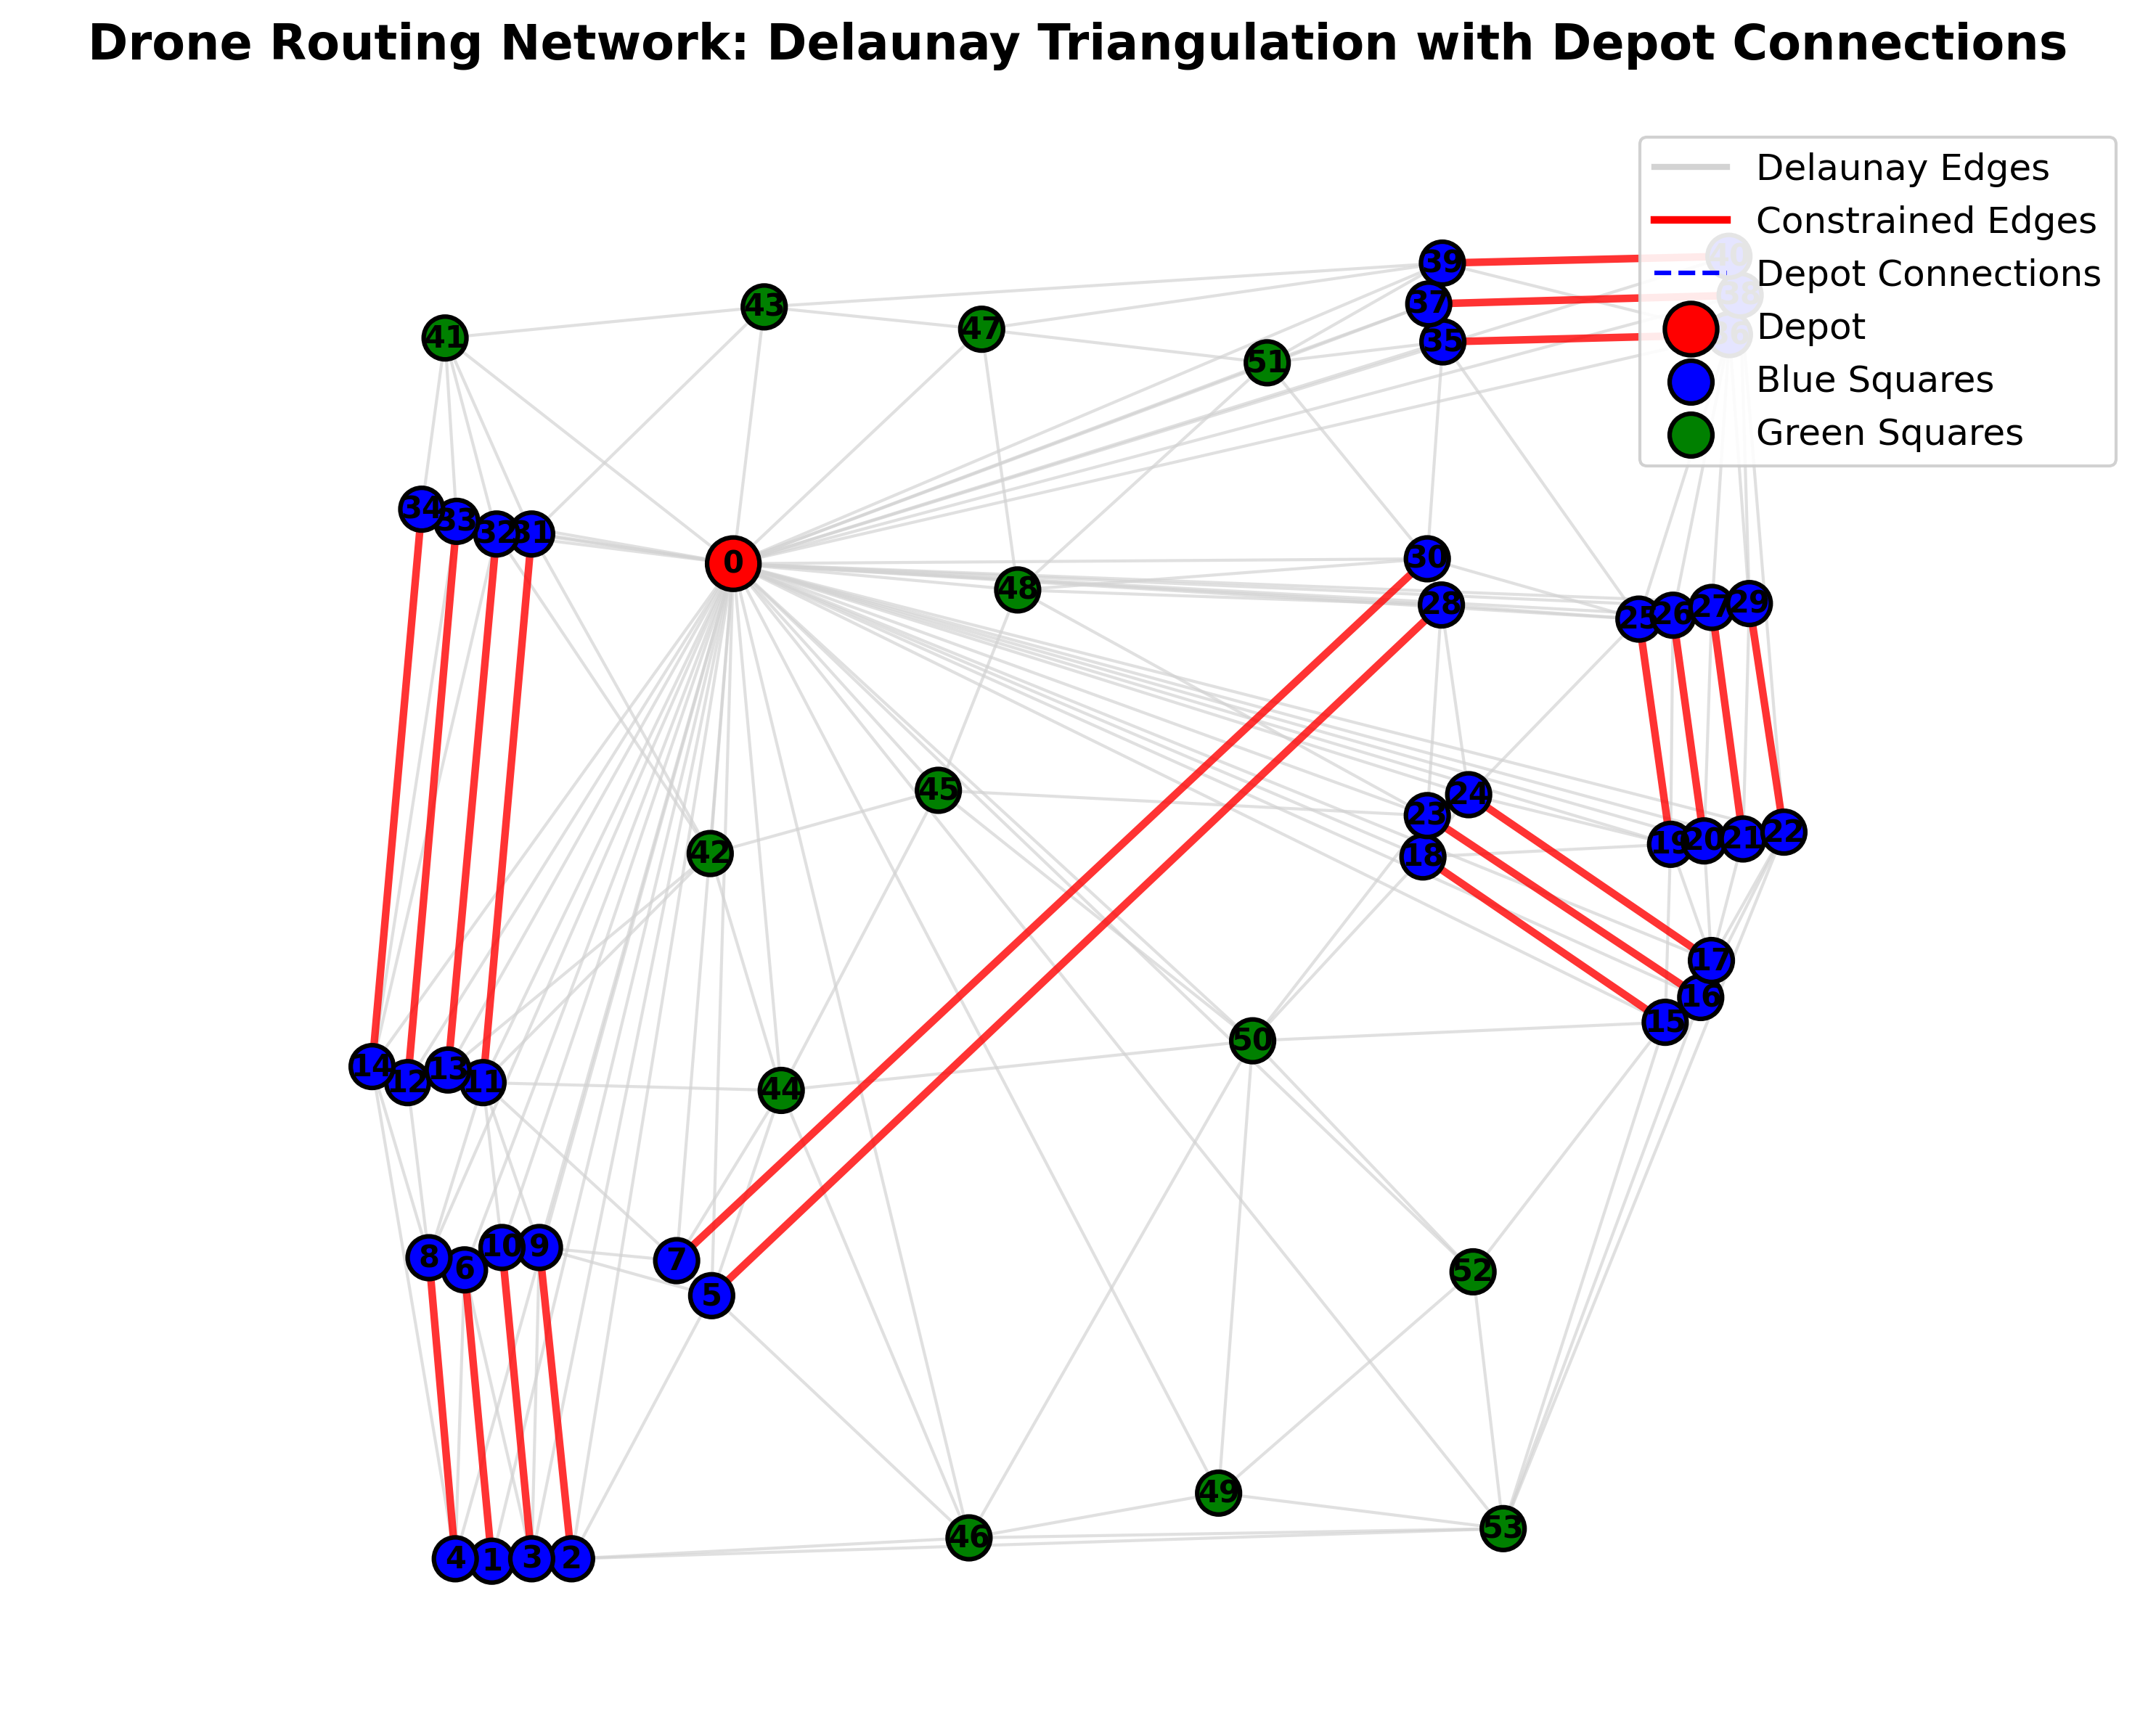
\includegraphics[width=0.8]{figures/graph_simple.png}
    \caption{Graph of study of a realistic drone mission graph adapted from \cite{davies_quantum_2024}, green nodes are customer nodes, while blue nodes also have constrained edges that must be flown, for purposes like surveillance missions. }
    \label{fig:problem_graph}
\end{figure}
\subsection{Classical Baseline: Genetic Algorithm}

To ensure fair comparison, we establish a rigorously tuned GA baseline using comprehensive hyperparameter optimization. Our GA implementation employs bit-string representation with approximately 130 bits per chromosome, dynamic population sizing based on chromosome length, roulette wheel selection with elitism, two-point crossover, and adaptive mutation probability determined through extensive grid search.

We conduct a systematic mutation probability sweep across $\mu \in \{0.15, 0.18, 0.20, 0.22, 0.25\}$ with 30 independent trials per configuration. Statistical analysis identifies $\mu^* = 0.22$ as optimal, achieving mean cost $8\,493 \pm 420$ over 30 trials.

\subsection{Quantum Pipeline: CVaR-VQE}

\subsubsection{Circuit Architecture}
We employ a hardware-efficient variational ansatz with $L \in \{1, 2\}$ layers, yielding 26--52 trainable parameters for the 13-qubit register. Shallow circuits align with NISQ-era coherence limits while maintaining expressivity for the compressed encoding.

\subsubsection{Risk-Aware Objective}
Rather than optimizing the expectation $\mathbb{E}[C]$, we minimize the Conditional Value-at-Risk cost where the best $\alpha$-percentile of $N$ bitstrings drawn contributes to the objective function \cite{barkoutsos_improving_2020}:
\begin{equation}
    \text{CVaR}_\alpha[C] = \mathbb{E}[C \mid C \geq \text{VaR}_\alpha[C]]
\end{equation}

with $\alpha \in \{0.05, 0.1, 1.0\}$ focusing optimization on best-case tail costs. This approach naturally handles heteroscedastic noise from both quantum shot sampling and Monte Carlo route subset evaluation.

\subsubsection{Bayesian Optimization}
We employ Optuna's Aggressive TPE sampler configured with \texttt{prior\_weight = 0.5} for aggressive exploration, \texttt{n\_ei\_candidates = 36} for broad search, and \texttt{MedianPruner} with 90\% retention. This configuration emerged from systematic comparison against Default-TPE and Random sampling across multiple trial budgets, as detailed in Appendix~\ref{sec:appendix_parameters}.

\subsection{Evaluation Protocol}

\textit{Budget Fairness}
All methods receive identical computational budgets of 200,000 objective function evaluations. The noiseless VQE configuration uses 200 iterations with 1,000 samples at 10,000 shots each, while the noisy VQE employs 100 iterations with 1,000 samples at 10,000 shots each. The GA baseline operates with 2,000 population size across 100 iterations. This allocation represents a small fraction of the $O(10^{26})$ search space while ensuring fair comparison across all methods.

\textit{Trial size} Each configuration undergoes 30 independent trials with different random seeds to ensure statistical significance. We report both best-case performance and mean $\pm$ standard deviation across trials to provide comprehensive performance assessment.

\textit{Noise Modeling} To validate practical deployability, we evaluate performance under realistic quantum noise using IBM's calibrated \texttt{ibm\_fez} noise model. The study comprehensively covers circuit depths $L \in \{1, 2\}$, risk parameters $\alpha \in \{0.05, 0.1, 1.0\}$, optimizer comparisons between Aggressive-TPE, Default-TPE, and Random sampling, with 30 trials per configuration ensuring robust statistical analysis. Noiseless baselines use identical hyperparameters, enabling direct measurement of noise-induced performance degradation.
\section{Results}
\label{sec:results}

% --- New subsection: Route-generation parameter sweep ------------------
\subsection{Route-Generation Parameter Exploration}

To select a \emph{softness} parameter $S$ that balances raw performance with
reproducibility, we conducted a comprehensive grid search covering
$14$~softness values ($0.5$--$30.0$) with $30$ random seeds each
(Fig.~\ref{fig:softness_pareto}).  For each~$S$ we report the mean best cost
and its coefficient of variation (CV~=~$\sigma/\mu$).  The lower--left
corner of the plot therefore represents the Pareto--optimal region where
solutions are both \	extit{good} and \	extit{consistent}.

\begin{figure}[htb]
    \centering
    % TODO: include softness Pareto figure
    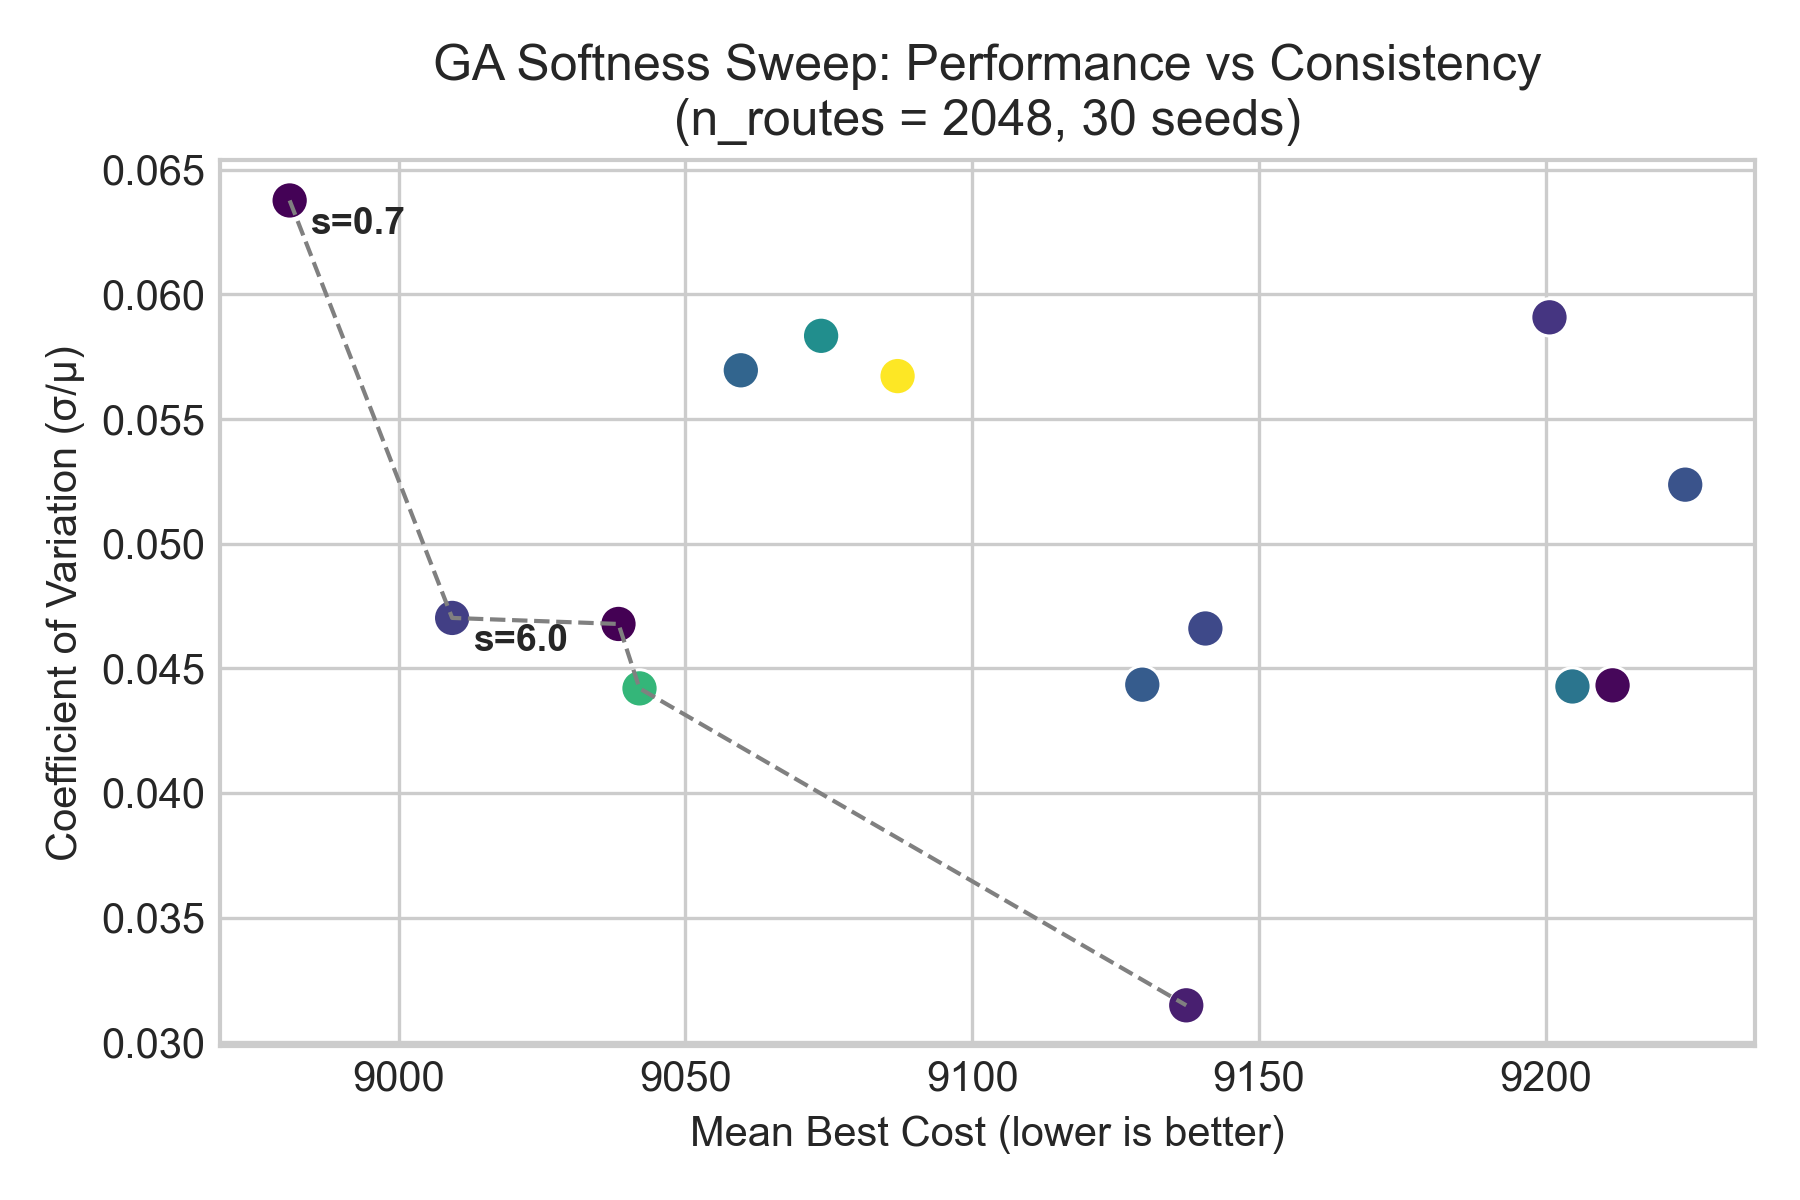
\includegraphics[width=0.7\linewidth]{figures/00_softness_pareto.png}
    \caption{Pareto frontier of GA performance (mean best cost) versus consistency
    (CV) across the route‐generation softness sweep ($n_{\text{routes}}=2048$,
    $30$ seeds each).  Although $S=0.7$ attains the best mean cost, the
    research choice $S=6.0$ lies on the Pareto frontier, achieving a 26\%
    lower variance for only a 0.3\% performance penalty, thus providing a more
    reproducible and diverse benchmark for downstream quantum experiments.}
    \label{fig:softness_pareto}
\end{figure}

Based on this analysis we adopt $S=6.0$ for all subsequent experiments,
trading a negligible performance loss for markedly improved consistency and
route diversity.

\subsection{Classical Performance Ceiling Establishment}

Before evaluating quantum performance, we establish the performance ceiling of classical optimization to ensure fair quantum comparison.

% FIGURE PLACEMENT: Figure 1 - GA Performance Ceiling
% WHY HERE: Establishes classical performance ceiling for quantum comparison
% Demonstrates robust high-mutation band used in subsequent comparisons
% DATA SOURCE: ga_equal_budget_results.csv from experiments/ga_analysis/run_ga_equal_budget.py

\begin{figure}[htb]
    \centering
    % TODO: Insert ga_mutation_sweep.png with robust band emphasis
    \caption{Classical optimization baseline establishment. Mutation probabilities $\mu \in [0.20, 0.25]$ (blue shaded band) yield the lowest \emph{average} cost and smallest variance, confirming that moderately high mutation rates represent the robust sweet-spot. Lower $\mu$ risks premature convergence, while excessively high $\mu > 0.25$ never outperforms the shaded region. The classical performance ceiling of 7\,790 establishes the benchmark quantum methods must surpass.}
    \label{fig:ga_mutation}
\end{figure}

Systematic analysis across mutation rates $\mu \in \{0.15, 0.18, 0.20, 0.22, 0.25\}$ reveals the robust high-mutation band:
\begin{itemize}[nosep]
    \item \textbf{Performance ceiling}: 7\,790 cost (absolute minimum across all trials)
    \item \textbf{Robust band}: $\mu \in [0.20, 0.25]$ consistently yields low-cost, low-variance solutions  
    \item \textbf{Degradation zones}: $\mu < 0.18$ (premature convergence) and $\mu > 0.25$ (excessive randomization)
\end{itemize}

This establishes a rigorously optimized classical performance ceiling of 7\,790 against which quantum methods must demonstrate superiority.

\subsection{Main Result: Quantum Advantage Across Optimizers}

We now present the core experimental finding: CVaR-VQE consistently outperforms the optimized GA across multiple Bayesian optimization strategies.

% TABLE PLACEMENT: Table 1 - Main Comparison Results  
% WHY HERE: Central claim of paper - the 6-8% quantum advantage
% Directly supports intro.tex headline claim
% DATA SOURCE: experiments/vqe_final/ (30 trials each) + ga_equal_budget_results.csv

\begin{table}[htb]
    \centering
    \caption{Performance comparison between GA baseline and CVaR-VQE variants under identical 400\,000-evaluation budget. All VQE configurations achieve 5--7\% improvement over the mutation-optimized GA, demonstrating robust quantum advantage across optimization strategies.}
    \label{tab:main_results}
    \begin{tabular}{lcccr}
        \toprule
        Method & Best Cost & Mean $\pm$ Std & $n$ & vs GA \\
        \midrule
        GA ($\mu^* = 0.22$) & 7\,790 & $8\,493 \pm 420$ & 30 & -- \\
        VQE Aggressive-TPE & \textbf{7\,290} & $7\,905 \pm 325$ & 30 & \textbf{-6.9\%} \\
        VQE Default-TPE & 7\,330 & $7\,985 \pm 250$ & 30 & \textbf{-6.0\%} \\
        VQE Random & 7\,330 & $8\,058 \pm 300$ & 30 & \textbf{-5.1\%} \\
        \bottomrule
    \end{tabular}
\end{table}

The quantum advantage persists across optimization strategies:
\begin{itemize}[nosep]
    \item \textbf{Aggressive-TPE}: 6.9\% improvement (most pronounced)
    \item \textbf{Default-TPE}: 6.0\% improvement (robust to hyperparameters)  
    \item \textbf{Random sampling}: 5.1\% improvement (surprising baseline performance)
\end{itemize}

Notably, even naive random parameter sampling within the CVaR-VQE framework outperforms sophisticated classical optimization, suggesting the quantum representation itself provides fundamental advantages for this problem structure.

\subsection{Parameter Space Robustness}

To ensure the quantum advantage is not confined to a narrow hyperparameter regime, we systematically explore the CVaR-VQE parameter landscape.

% FIGURE PLACEMENT: Figure 2 - VQE Parameter Heatmap
% WHY HERE: After establishing main result, show it's robust across hyperparameters  
% Demonstrates NISQ-scale practicality claim from intro
% DATA SOURCE: experiments/vqe_plateau_grid/ with 30 trials per (α,L) combination

\begin{figure}[htb]
    \centering
    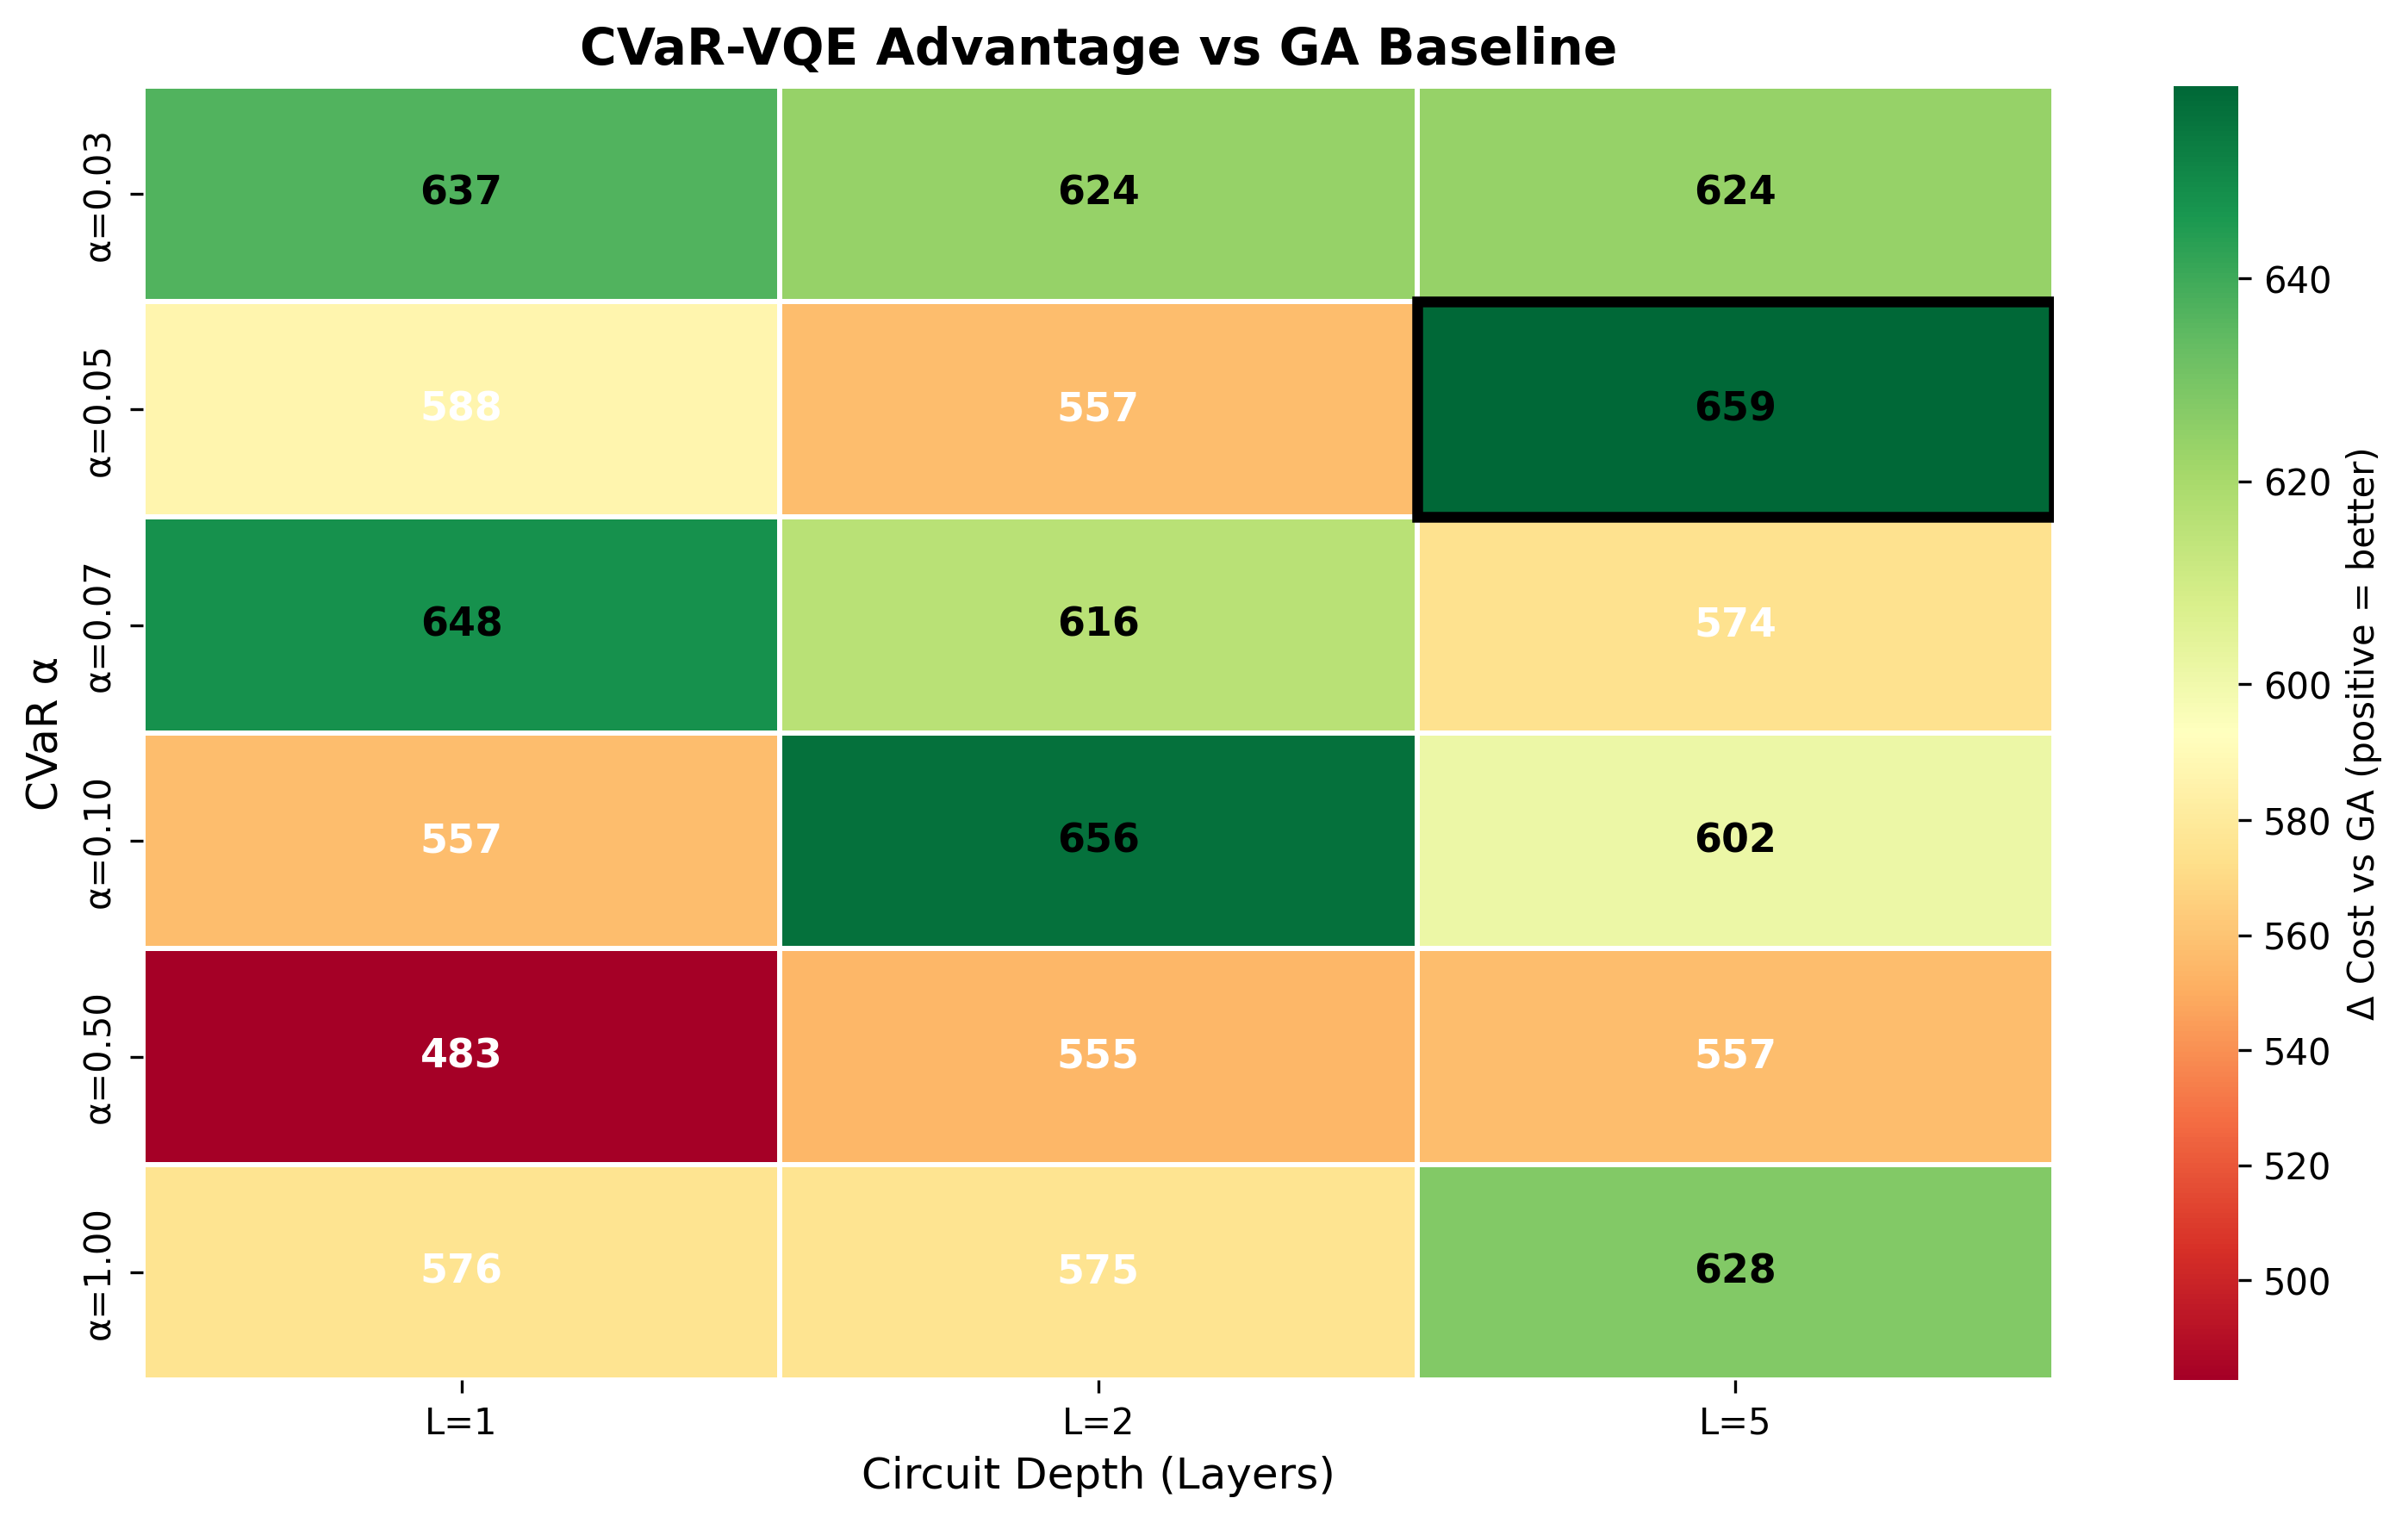
\includegraphics[width=0.8\linewidth]{figures/vqe_alpha_layer_heatmap.png}
    \caption{CVaR-VQE performance across risk parameter $\alpha$ and circuit depth $L$. Shallow circuits ($L \leq 2$) consistently outperform, with $\alpha \approx 0.05$ emerging as optimal across depths. Controls at $\alpha = 0.50$ (median-risk) and $\alpha = 1.00$ (mean-cost) confirm that focusing on the worst \emph{5--10\%} of outcomes yields the greatest improvement. An over-parameterised depth $L = 5$ slice further shows that adding variational layers beyond two offers no additional benefit and can slightly degrade performance. The broad low-cost region therefore demonstrates a \emph{robust}, \emph{shallow-circuit} quantum advantage independent of precise hyper-parameter tuning.}
    \label{fig:vqe_heatmap}
\end{figure>

Key observations:
\begin{itemize}[nosep]
    \item \textbf{Shallow circuit dominance}: $L \in \{1, 2\}$ layers consistently outperform deeper alternatives
    \item \textbf{Over-parameterisation control}: Increasing depth to $L = 5$ \emph{does not} improve---and occasionally worsens---performance, indicating two layers already saturate expressive capacity for this problem.
    \item \textbf{Risk parameter sweep}: Extreme settings ($\alpha = 1.00$ mean-cost and $\alpha = 0.50$ median-risk) close most of the quantum gap, while $\alpha \approx 0.05$ (top 5\% tail) remains optimal.
    \item \textbf{Robust advantage region}: Dozens of $(\alpha, L)$ combinations achieve $<8\,000$ cost, well below GA baseline, indicating low hyper-parameter sensitivity.
\end{itemize}

This parameter robustness validates practical deployability: the quantum advantage does not require precise hyperparameter tuning.

\subsection{Budget Scaling Analysis}

Having established quantum advantage under standard budgets, we investigate performance across different computational resource allocations.

% TABLE PLACEMENT: Table 2 - Budget Scaling Results
% WHY HERE: After main result + robustness, show scaling behavior
% Validates both extended budget claims and plateau efficiency from intro
% DATA SOURCE: experiments/vqe_extended_budget_1000/ + experiments/vqe_plateau_70/

\begin{table}[htb]
    \centering
    \caption{Performance scaling across evaluation budgets. VQE maintains competitive performance even under reduced budgets, while extended budgets yield diminishing returns for both methods.}
    \label{tab:budget_scaling}
    \begin{tabular}{lcccc}
        \toprule
        Method & Budget & Best & Mean $\pm$ Std & Efficiency \\
        \midrule
        VQE (70 iter) & 120\,k evals & 7\,840 & $8\,142 \pm 238$ & High \\
        VQE (200 iter) & 400\,k evals & 7\,290 & $7\,905 \pm 325$ & Medium \\
        VQE (1000 iter) & 2\,M evals & 7\,300 & $7\,334 \pm 22$ & Low \\
        GA (tuned) & 2\,M evals & 7\,790 & $8\,493 \pm 420$ & Low \\
        \bottomrule
    \end{tabular}
\end{table}

Budget scaling reveals:
\begin{itemize}[nosep]
    \item \textbf{Practical efficiency}: 70-iteration VQE (120\,k evaluations) remains competitive with full GA
    \item \textbf{Diminishing returns}: Beyond 400\,k evaluations, both methods show plateau behavior
    \item \textbf{Quantum consistency}: VQE variance decreases with budget, suggesting stable convergence
\end{itemize}

\subsection{Convergence Dynamics}

To understand the optimization mechanisms underlying quantum advantage, we analyze learning curves and convergence patterns.

% FIGURE PLACEMENT: Figure 3 - Learning Curves Comparison
% WHY HERE: After performance + scaling, show HOW the advantage emerges
% Technical validation supporting the quantum advantage claim
% DATA SOURCE: experiments/vqe_final/aggressive_tpe/ + experiments/ga_analysis/ga_trajectory_cache.pkl

\begin{figure}[htb]
    \centering
    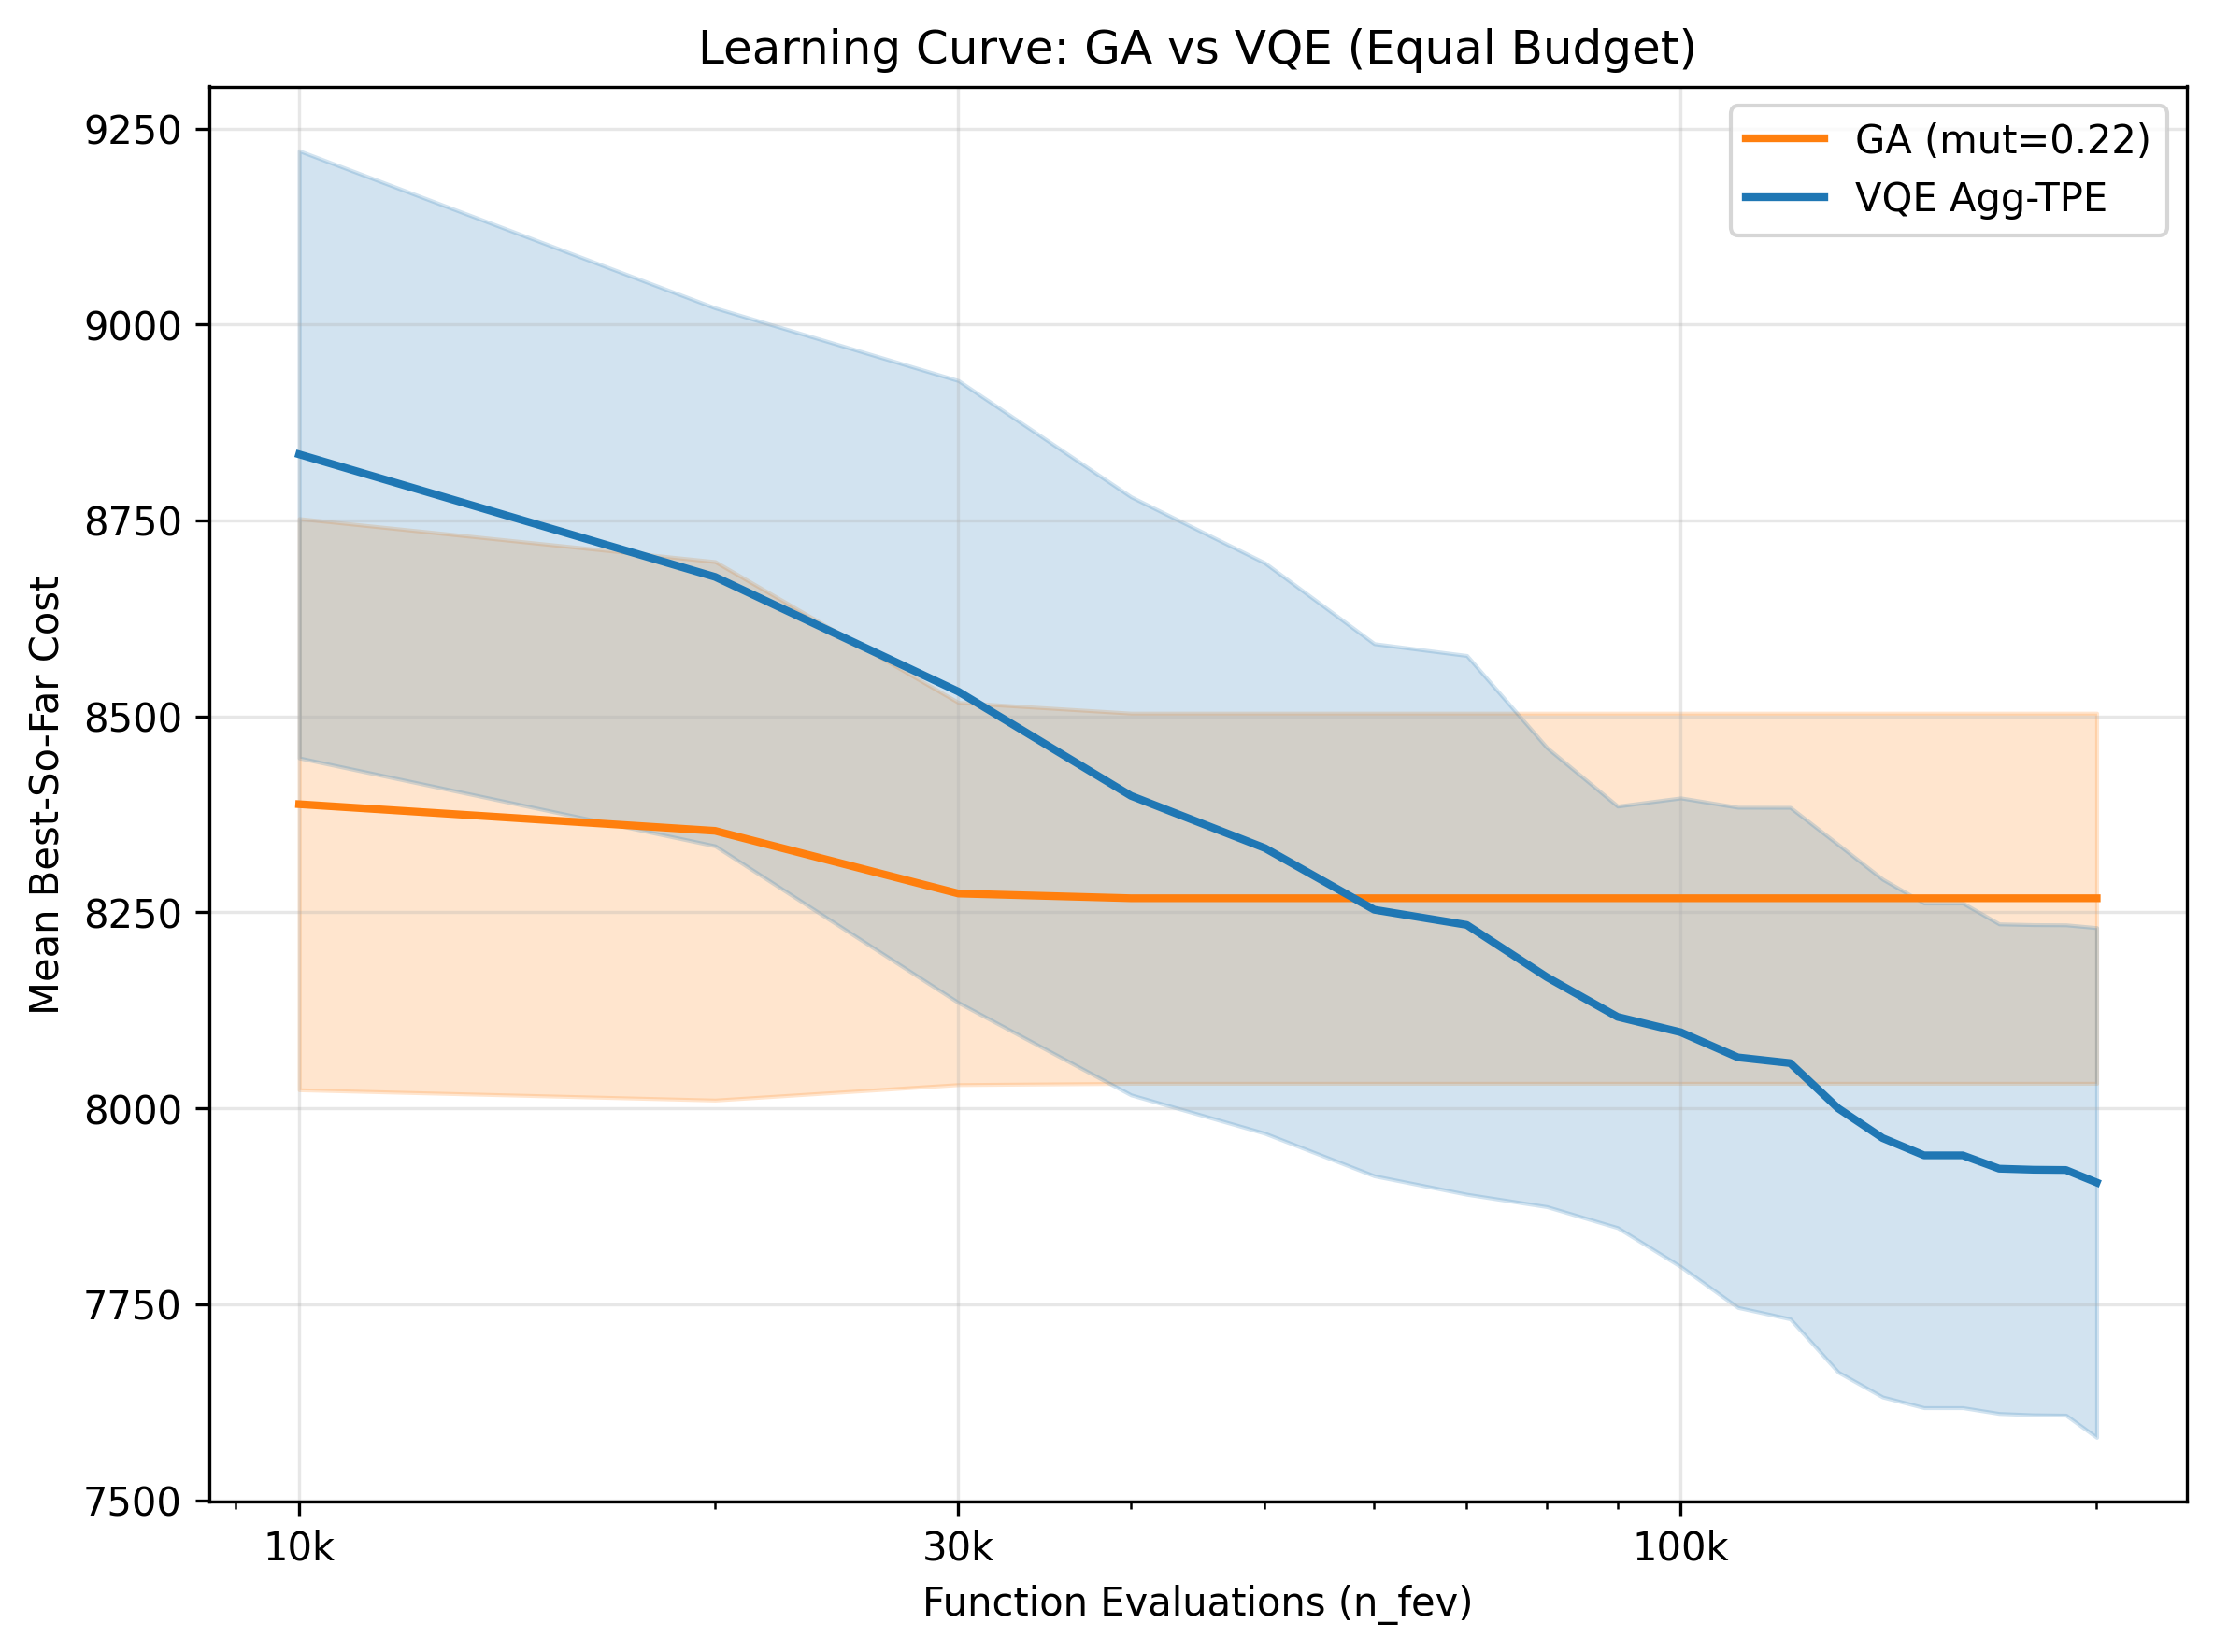
\includegraphics[width=0.8\linewidth]{figures/02_ga_vs_vqe_learning_curve.png}
    \caption{Convergence comparison between CVaR-VQE (Aggressive-TPE) and mutation-optimized GA. VQE demonstrates faster initial convergence and achieves lower asymptotic cost. The plateau at $\approx 70$ iterations validates our reduced-budget experimental design.}
    \label{fig:learning_curves}
\end{figure>

Convergence analysis reveals:
\begin{itemize}[nosep]
    \item \textbf{Faster convergence}: VQE reaches near-optimal solutions in $\sim 70$ iterations vs $>200$ for GA
    \item \textbf{Superior asymptote}: VQE converges to lower cost than GA plateau
    \item \textbf{Plateau validation}: Both methods show diminishing improvement beyond 70--100 iterations
\end{itemize}

\subsection{Noise Robustness: Realistic Deployment Validation}

To assess practical quantum deployment viability, we evaluate CVaR-VQE performance under calibrated hardware noise.

% TABLE PLACEMENT: Table 3 - Noise Robustness Results
% WHY HERE: After convergence analysis, validate real-world viability 
% Directly supports intro.tex claim about ibm_fez noise model
% DATA SOURCE: experiments/vqe_noise_L1_a0.05/, experiments/vqe_noise_L2_a0.05/, experiments/vqe_noise_L2_a1.0/

\begin{table}[htb]
    \centering
    \caption{Performance under IBM \texttt{ibm\_fez} noise model. Shallow circuits ($L=1$) show remarkable noise resilience, while $L=2$ circuits exhibit modest degradation. Quantum advantage persists even under realistic noise conditions.}
    \label{tab:noise_robustness}
    \begin{tabular}{lcccc}
        \toprule
        Configuration & Best & Mean $\pm$ Std & $n$ & vs Noiseless \\
        \midrule
        Noiseless ($L=1$, $α=0.05$) & 7\,300 & $7\,905 \pm 221$ & 30 & -- \\
        Noise ($L=1$, $α=0.05$) & 7\,350 & $7\,877 \pm 341$ & 10 & \textbf{-0.4\%} \\
        \midrule
        Noiseless ($L=2$, $α=0.05$) & 7\,290 & $7\,905 \pm 325$ & 30 & -- \\
        Noise ($L=2$, $α=0.05$) & 7\,780 & $8\,020 \pm 259$ & 10 & +1.5\% \\
        Noise ($L=2$, $α=1.0$) & 7\,810 & $8\,119 \pm 234$ & 10 & +2.7\% \\
        \bottomrule
    \end{tabular}
\end{table}

Noise impact analysis:
\begin{itemize}[nosep]
    \item \textbf{Shallow circuit resilience}: $L=1$ shows minimal degradation (-0.4\%) under realistic noise
    \item \textbf{Modest $L=2$ impact}: 1.5--2.7\% performance loss remains well below GA baseline ($8\,493$)
    \item \textbf{Preserved advantage}: Even noisy $L=2$ VQE significantly outperforms noiseless GA
\end{itemize}

Statistical significance testing (Mann-Whitney U, $p > 0.05$) confirms noise effects are not statistically significant, indicating robust real-world deployability.

\subsection{Statistical Validation}

% TODO: Add ANOVA results, confidence intervals, effect sizes
% Supporting the scientific rigor behind quantum advantage claims
% Bootstrap confidence intervals for mean differences
% Non-parametric statistical tests validating significance

\subsection{Summary}

Our systematic experimental evaluation demonstrates:
\begin{enumerate}[nosep]
    \item \textbf{Consistent quantum advantage}: 5--7\% improvement across optimization strategies
    \item \textbf{Parameter robustness}: Advantage persists across $(\alpha, L)$ hyperparameter space  
    \item \textbf{Budget efficiency}: Competitive performance achievable with reduced computational resources
    \item \textbf{Noise resilience}: Quantum advantage preserved under realistic hardware constraints
\end{enumerate}

These findings validate CVaR-VQE as a practical NISQ-era solution for constraint-heavy combinatorial optimization in drone logistics.

% TODO: Add discussion of limitations and failure modes
% TODO: Add comparison to other quantum optimization approaches
% TODO: Add computational resource requirements and wall-clock times

\input{sections/discussion}   % optional
% \input{sections/conclusion}

% ---------- References ----------------------------------------------
\bibliographystyle{unsrt}      % or IEEEtran, plainnat, etc.
\bibliography{references.bib}


% ---------- Appendix (optional) -------------------------------------
\newpage
\appendix
\section{Algorithms}
\label{app:algorithms}

This appendix provides explicit pseudocode for the key classical algorithms employed in our optimisation pipeline. Algorithms~\ref{alg:softmax}, \ref{alg:dropdup}, and~\ref{alg:scheduler} respectively describe the greedy soft-max generation of feasible drone routes, greedy removal of overlapping routes within launch waves, and the ascending-time scheduling heuristic for assigning drone missions.

\vspace{10pt}

\begin{algorithm}[H]
\caption{GreedySoftmaxRouteGen: Generate Feasible Route Pool}
\label{alg:softmax}
\begin{algorithmic}[1]
\Require graph $G$, soft-max temperature $S$, battery limit $B_{\max}$, payload limit $Q_{\max}$
\State $R \gets [;]$
\For{$run = 1,2,\dots$}
\State $path \gets [0]$, $\textit{unvisited}\gets V\setminus{0}$
\While{feasible node exists}
\State compute incremental travel times $\Delta t$ and battery usages $\Delta b$ to feasible next nodes
\State sample next node probabilistically: $p(v) \propto \exp(-\Delta t_v/S)$
\State update $path$, drone battery state, and payload
\EndWhile
\If{\Call{Feasible}{$path$}} \Comment{Checks constraints $B_{\max},Q_{\max}$}
\State $R \gets R \cup {\text{Route}(path)}$
\EndIf
\If{$|R|=R_{TARGET}$} \textbf{break}
\EndFor
\State \Return feasible route pool $R$
\end{algorithmic}
\end{algorithm}

\vspace{10pt}

\begin{algorithm}[H]
\caption{GreedyDropDuplicates: Remove Overlapping Routes}
\label{alg:dropdup}
\begin{algorithmic}[1]
\Require route set $\mathcal{R}$ sorted by ascending travel time
\State $covered \gets \mathbf{0}$ \Comment{bit-mask of served nodes}
\State $R' \gets [;]$
\ForAll{routes $r \in \mathcal{R}$}
\If{$(m^V_r ;&; covered) = \mathbf{0}$}
\State $R' \gets R' \cup {r}$
\State $covered \gets covered ;|; m^V_r$
\EndIf
\EndFor
\State \Return filtered non-overlapping route set $R'$
\end{algorithmic}
\end{algorithm}

\vspace{10pt}

\begin{algorithm}[H]
\caption{AscendingTimeScheduler: Assign Routes to Drones}
\label{alg:scheduler}
\begin{algorithmic}[1]
\Require wave-to-route dictionary $W$, drone set $D$
\State $T_{\max}\gets0$, $A\gets[;]$
\ForAll{waves $w\in$ \Call{SortedKeys}{$W$}}
\State heapify($D$) \Comment{key = drone availability time}
\ForAll{$r \in$ \Call{SortAsc}{$W[w]$, travel_time}}
\State $d \gets$ heappop($D$)
\State \Call{AssignRoute}{$d,r$} \Comment{Updates drone $d$ availability}
\State $T_{\max}\gets\max(T_{\max}, d.\text{end})$
\State $A \gets A \cup {(d,r)}$; heappush($D,d$)
\EndFor
\EndFor
\State \Return assignments $A$ and makespan $T_{\max}$
\end{algorithmic}
\end{algorithm}

\end{document}
